\problemname{Wind Turbines}

Anna has been tasked with designing the wiring for a new offshore wind farm in the North Sea consisting of $N$ turbines, numbered $0, 1, \ldots, N-1$. Her goal is to ensure that all turbines are connected to the shore as cheaply as possible.

Anna has a list of $M$ potential connections, each linking two wind turbines and having a specific cost. Additionally, the nearby city has agreed to cover the costs of connecting a consecutive interval $[\ell, r]$ of turbines to the shore. That is, each turbine $t$ in this range ($\ell\le t\le r$) is directly connected to the shore for free. 
If all potential connections are built, there is a way to reach any wind turbine from any other wind turbine.
That implies that as soon as one of the wind turbines is connected to the shore, it is possible to build connections such that the power from all the turbines can be transferred to the shore. Of course, more connections to the shore may allow for a cheaper total cost.
Note that the free connections are the only direct ones to the shore.

It is Anna's job to select a subset of the potential connections in a way that minimizes the sum of their costs, while ensuring that every wind turbine can reach the shore (possibly via other wind turbines).

In order to make an informed decision, the city provides Anna with $Q$ possible options for the interval $[\ell, r]$. The city asks Anna to compute the minimum cost for each of these scenarios.

\section*{Input}
The first line of the input contains three integers, $N$, $M$ and $Q$.

The following $M$ lines contain three integers each, $u_i$, $v_i$ and $c_i$. The $i$th line describes a potential connection between wind turbines $u_i$ and $v_i$ that has the cost $c_i$. These connections are undirected and connect two different turbines. No two connections are between the same pair of turbines.
It is guaranteed that, if all potential connections are built, any wind turbine is reachable from any other (directly or indirectly).

The next $Q$ lines contain two integers each, $\ell_i$ and $r_i$, describing the scenario where the shore directly connects to the wind turbines $\ell_i,\ell_i+1,\ldots,r_i$. Note that we can have $r_i = \ell_i$ when the shore directly connects to a single wind turbine.

\section*{Output}
Output $Q$ lines, one line per scenario, containing one integer each, the minimum cost of connecting the turbines such that every turbine can deliver its power to the shore.

\section*{Constraints and Scoring}
\begin{itemize}
\item $2 \le N\le 100\,000$.
\item $1 \le M\le 100\,000$.
\item $1 \le Q\le 200\,000$.
\item $0 \le u_i,v_i \le N-1$.
\item $u_i \ne v_i$, and there is at most one direct connection between each pair of wind turbines.
\item $1 \le c_i \le 1\,000\,000\,000$.
\item $0 \le \ell_i\le r_i \le N-1$.
\end{itemize}

Your solution will be tested on a set of test groups, each worth a number of points. Each test group contains a set of test cases. To get the points for a test group, you need to solve all the test cases in the test group.


\begin{tabular}{|l|l|l|}
\hline
Group  &  Score  &  Limits \\
\hline
 1 & 8 & $M=N-1$ and the $i$th connection has $u_i=i$ and $v_i=i+1$, i.e. if all connections are built, they form a path $0 \leftrightarrow 1 \leftrightarrow 2 \leftrightarrow \ldots \leftrightarrow N-1$   \\
\hline
  2 & 11 & $N,M,Q\le 2\,000$ and $\sum(r_i-\ell_i+1) \le 2\,000$   \\
\hline
  3 & 13 & $r_i=\ell_i+1$ for all $i$   \\
\hline
  4 & 17 & $1\le c_i \le 2$ for all $i$, i.e., each connection has cost either $1$ or $2$   \\
\hline
  5 & 16 & $\sum(r_i-\ell_i+1)\le 400\,000$   \\
\hline
  6 & 14 & $\ell_i=0$ for all $i$   \\
\hline
  7 & 21 & No additional constraints   \\
\hline
\end{tabular}
\section*{Examples}
In the first example, we are given the following graph of potential connections.

\begin{center}
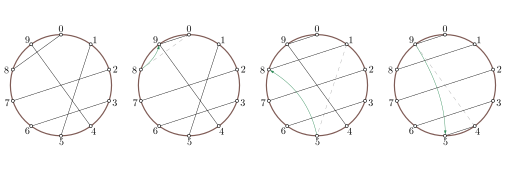
\includegraphics[width=0.3\textwidth]{sample1.pdf}
\end{center}
We are given three scenarios.
In the first scenario, turbine 1 is the only one with a connection to the shore. In this case, we need to keep all connections except for the connection between turbine $0$ and turbine $2$, giving a total cost of $2+3+6+3=14$.
In the next scenario, the turbines 3 and 4 are connected to the shore. In this case, we keep the connections $(1,0)$, $(1,2)$ and $(2,4)$, giving a cost of 8.
In the third scenario, all but turbine 0 are connected to the shore. In this case, we only need to connect this one to another turbine, which we do by choosing the connection $(0,1)$.
The solutions to the scenarios are depicted below:

\begin{center}
\begin{tabular}{p{0.3\textwidth} p{0.3\textwidth} p{0.3\textwidth}}
\includegraphics[width=\textwidth]{sample1q1} &
\includegraphics[width=\textwidth]{sample1q2} &
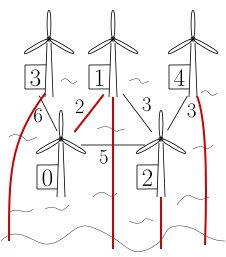
\includegraphics[width=\textwidth]{sample1q3} \\
\end{tabular}
\end{center}

The first and the sixth samples satisfy the constraints of test groups 2, 5 and 7. The second and the seventh samples satisfy the constraints of test groups 1, 2, 5 and 7. The third sample satisfies the constraints of test groups 2, 3, 5 and 7. The fourth sample satisfies the constraints of test groups 2, 4, 5 and 7. The fifth sample satisfies the constraints of test groups 2, 5, 6 and 7.


